\documentclass[onecolumn, draftclsnofoot,10pt, compsoc]{IEEEtran}
\usepackage{graphicx}
\usepackage{url}
\usepackage{setspace}
\usepackage[font=small,labelfont=bf]{caption} % Required for specifying captions to tables and figures
\usepackage{geometry}
\usepackage{listings}
\geometry{textheight=9.5in, textwidth=7in}

% 1. Fill in these details
\def \CapstoneTeamName{		Malsano}
\def \CapstoneTeamNumber{		72}
\def \GroupMemberOne{			Katherine Jeffrey}
\def \GroupMemberTwo{			Brandon Jolly}
\def \GroupMemberThree{			Bradford Wong}
\def \CapstoneProjectName{		App to Support Field Diagnostics in Veterinary Medicine}
\def \CapstoneSponsorCompany{	Oregon Veterinary Diagnostics Laboratory}
\def \CapstoneSponsorPerson{		Professor Christiane Loehr}

% 2. Uncomment the appropriate line below so that the document type works
\def \DocType{		%Problem Statement
				%Requirements Document
				%Technology Review
				%Design Document
				Progress Report
				}
			
\newcommand{\NameSigPair}[1]{\par
\makebox[2.75in][r]{#1} \hfil 	\makebox[3.25in]{\makebox[2.25in]{\hrulefill} \hfill		\makebox[.75in]{\hrulefill}}
\par\vspace{-12pt} \textit{\tiny\noindent
\makebox[2.75in]{} \hfil		\makebox[3.25in]{\makebox[2.25in][r]{Signature} \hfill	\makebox[.75in][r]{Date}}}}
% 3. If the document is not to be signed, uncomment the RENEWcommand below
\renewcommand{\NameSigPair}[1]{#1}

%%%%%%%%%%%%%%%%%%%%%%%%%%%%%%%%%%%%%%%
\begin{document}
\begin{titlepage}
    \pagenumbering{gobble}
    \begin{singlespace}
    	
\includegraphics[height=4cm]{coe_v_spot1}
        \hfill 
        % 4. If you have a logo, use this includegraphics command to put it on the coversheet.
        %\includegraphics[height=4cm]{CompanyLogo}   
        \par\vspace{.2in}
        \centering
        \scshape{
            \huge CS Capstone \DocType \par
            {\large\today}\par
            \vspace{.5in}
            \textbf{\Huge\CapstoneProjectName}\par
            \vfill
            {\large Prepared for}\par
            \Huge \CapstoneSponsorCompany\par
            \vspace{5pt}
            {\Large\NameSigPair{\CapstoneSponsorPerson}\par}
            {\large Prepared by }\par
            Group\CapstoneTeamNumber\par
            % 5. comment out the line below this one if you do not wish to name your team
            \CapstoneTeamName\par 
            \vspace{5pt}
            {\Large
                \NameSigPair{\GroupMemberOne}\par
                \NameSigPair{\GroupMemberTwo}\par
                \NameSigPair{\GroupMemberThree}\par
            }
            \vspace{20pt}
        }
        \begin{abstract}
        % 6. Fill in your abstract    
        	Currently, there are many difficulties for veterinary pathologists trying to perform remote diagnostics. There are not any effective ways for people out in the field collecting samples to communicate with specialized experts located in laboratories. As a result, this project will involve creating an Android mobile application that will be used as a bridge to connect the field personnel with the veterinary pathologists in laboratories. With this mobile application, the field personnel will be able to take pictures of the individual that is being analyzed and then send the pictures along with other data such as the patient, location, and time to a pathologist. The pathologist will then be able to use the provided information to perform a necropsy and send feedback to the field personnel. This project is intended to support remote field diagnostics in veterinary medicine.
        \end{abstract}     
    \end{singlespace}
\end{titlepage}
\newpage
\pagenumbering{arabic}
\tableofcontents
% 7. uncomment this (if applicable). Consider adding a page break.
%\listoffigures
%\listoftables
\clearpage

% 8. now you write!
\section{Project Purpose and Goals}
The completed project components are intended to serve as a means of communication between personnel in the field and pathologists in the laboratory. Thhe project's purpose is to improve a team's ability to perform remote diagnostics by providing a convenient way for teams to communicate information. The OVDL wants a native Android mobile application that collects field data and images, stores the information on a native SQLite database, sends the information to the lab’s MySQL database using an API provided by the client, and gets real time feedback from the lab. The lab can interact with the database and user's submissions through a website, but the website is a stretch goal.

\section{Progress and Plans}
\subsection{Completed Parts of Project}
\subsubsection{Database}
We have completed the implementation of the MySQL database and the SQLite database on the Android app. In MySQL, we have added all the required tables. We have changed the image table to be renamed as pictures to avoid any confusion with the image object in Android Studio. All of the necessary primary key constraints have been included in each table. Each of the table has the required foreign key constraints for that table. For example, the PICTURE table has a foreign key from the SUBMISSION table. This code is shown in Figure 1. 

The SQLite database also has the required tables implemented. They do not have any foreign key constraints because this is handled by the Android programming. It will then be further checked once the information is sent to the MySQL database through the use of the client's API. The android app has the required procedures to insert data into the SQLite database, and to grab information from the tables to be displayed to the user. 

\subsubsection{Android}
The home screen has been completely implemented. All of the navigation buttons have been added and they all take the user to the corresponding screens. Additionally, the toolbar has been implemented and can take the user to any of the relevant screens.

Clicking on the "Create Account" button successfully opens up a web browser. It takes the user to the registration page on the website.

For the create submissions screen, all of the input fields were added. The "Save Draft" and "Submit" buttons correctly store the submission data into the SQLite database. Additionally, the "Add Pictures" screen has been implemented. Users can upload up to five pictures using either the camera or the phone's gallery and can also delete the pictures they uploaded. Also, the application can track all of the meta data of the pictures, including the name of the picture, the date it was taken, and the GPS coordinates. Users can also navigate to the "Add Samples" screen where they can add information about their samples. They can add as many samples as they want and can delete them as well. Clicking on the check mark button on the "Add Samples" and "Add Pictures" screen will save the pictures and samples.

For the "View Drafts" screen, all of the drafts stored in the database can be seen in a list. Additionally, users can remove drafts from the database by long clicking on the entry in the list. Clicking on one of the drafts in the list will navigate the user to the "Create Submission" screen. The information that the user entered before saving the draft will be automatically filled out for the user.

For the "View Submissions" screen, the user can view all of the submissions that they submitted to the database in a list. The user can also click on an entry and the app will successfully navigate to that submission's detailed page. The detailed page shows all of the information the user entered when creating the submission. This includes the title of the submission, group name, date the submission was created, the comment, the sick element, pictures, and samples. Like the View Drafts screen, the user can delete submissions from the database by long clicking on the submission in the list. Each entry in the list also shows the relevant information such as the submission title, the case ID, and when the submission was created.

Clicking on the "Instructions" button on the toolbar will take the user to the "Instructions" screen. This screen tells the user how to use the app and the contact information of the OVDL.

Clicking on the "Settings" option in the toolbar will navigate the user to the "Settings" screen. On this screen, users can log in and log out by clicking on the corresponding buttons. If the users try to create a submission without being logged in, the app will prompt the user to log in first. 

\subsubsection{Website}
Although the website is a stretch goal, the team had time to work on parts of the website. All the pages of the website have been created with basic layouts. The main page is the submissions page that has a table of all the submissions available to the user. The table shows the submission title, the name of the user that submitted it, its case ID and the date it was received. When clicked the individual submissions open a case detail page with the rest of the submission data. This is where messages will be processed. Users will be able to send messages about the submission to the submitter's phone and see any replies. 

There is also an account page where users can see and change their username or password. An about page is also included to provide users with information about the site, the app, and how to use them or contact people who can assist them. The pages are all accessible to each other though a navigation bar at the top of the pages. The website is currently hosted on the client's server and the domain name is myvetpath. It will be connected to the database with an API provided by the client. 


\subsection{Parts of Project Left to Complete}
\subsubsection{Database}
For both databases we will need final confirmation on any names of the table. We will also need to do some field test with their information to insure we are not missing any information during collection. We would need to create any views the client will need to make it easier for the API to query information once it has been completed. We also need to test to insure the API is properly sending information to the MySQL Database. This also means we need to test to the other direction as well. Those are the major things we need to add to the Database, with a few bug fixes along the way. 
\subsubsection{Android}
The Android app has all the required core functionality except for the tasks that use the API. These tasks aren't complete yet because the client promised the team that he would create the API, but he is still developing it at the moment. As a result, the team hasn't been able to work on any tasks that involve it. This includes authenticating log in credentials, sending 
data from the phone to the server, and receiving comments on submissions from the MySQL database. Lastly, there are some bugs involving drafts and the toolbar that need to be fixed.

\subsubsection{Website}
The website is still a stretch goal that the team would like to continue to work on in the future. The website has not been connected to the database because the API is still being developed by the client. Once it is ready to connect, some choices about the login and registration process will need to be made. The clients will need to decide how much security is necessary and specify the differences between user groups. We have discussed having levels of privileges for general users, OVDL affiliated users, and OVDL veterinary pathologist users. It is still unclear how security levels will be assigned and enforced. 

Another important piece that is sill unclear is messaging. We know pathologists will need to send messages to users about their submissions, but it is unclear if pathologists will also send messages to each other or how security levels will affect the messaging system. Unstable network connectivity is also a concern so we will need to implement a way of handling potential internet interruptions. 

\section{Problems}
The first issue we had was one of our team members was unable to push anything to our Android repository. He was able to pull information but when he tried to push it would say he did not have authorization. We checked the repository to see if he was added as a collaborator. That was not the issue. We met as a group to see what was wrong. We had him reinstall Android studio and tried switching Github accounts. We eventually figured out that the issue was that his laptop kept autofilling one of his other Github accounts information.

An issue we had during testing the submissions table in our SQLite database was that any changes we made to the SQLite submission table would not be shown in the Android emulator. We tried using different emulators, but the same error would occur. The solution was that we needed to recreate the tables for the changes to occur. It did enforce our belief the database was not being created every time we opened the app though.

A permission issue we all had was connecting to the MySQL database from outside the server. If we used putty, we could get to the server and interact with the tables but we could not interact with the table without using putty. We tried direct connections but we kept getting errors stating we did not have permission. The solution this time was found out by our client, who discovered we needed to create an ssh tunnel on the server in order for us to connect outside of it. Once this was created we had no more problems connecting.

When we were testing to see if we could add submissions to the SQLite database we could not figure out why any new additions could not be displayed. We used logs to see the flow of how a submission was processed in our app and determined it was being added correctly, but we simply could not retrieve the information that was stored. With the help of the logs we then determined to look deeper into the function used to retrieve the data from the SQLite server. Turns out the function had a logic error and was trying to display something that could not happen. Once we fixed the logic problem in the function, the submissions were properly displaying.

Another issue that we had was that we haven't been able to use the API yet because the client is still developing it. As such we have not been able to test the connection between the Android app and the database sever and we haven't been able to complete any API related tasks. Since we finished the rest of the core functionality early, we tried to assist him with the API, but we are still having problems with retrieving data from the MySQL database.\newline\newline

%added new lines to insure section 4 was next to it's contents.
\section{Code and Images}

\begin{lstlisting}
CREATE TABLE `PICTURE` (
  `ImageID` int(11) NOT NULL,
  `MasterID` int(11) NOT NULL,
  `ImagePath` varchar(255) NOT NULL,
  `Title` varchar(255) DEFAULT NULL,
  `Latitude` bigint(20) NOT NULL,
  `Longitude` bigint(20) NOT NULL,
  `DateTaken` date NOT NULL,
  PRIMARY KEY (`ImageID`,`MasterID`),
  KEY `MasterID idx` (`MasterID`),
  CONSTRAINT `MasterIDForPicture` FOREIGN KEY (`MasterID`) REFERENCES `SUBMISSION` (`MasterID`) 
  ON DELETE NO ACTION 
  ON UPDATE NO ACTION
) ENGINE=InnoDB DEFAULT CHARSET=latin1; 
\end{lstlisting}
\captionof{figure}{Code to create PICTURE Table in the MySQL Database}

\begin{center}
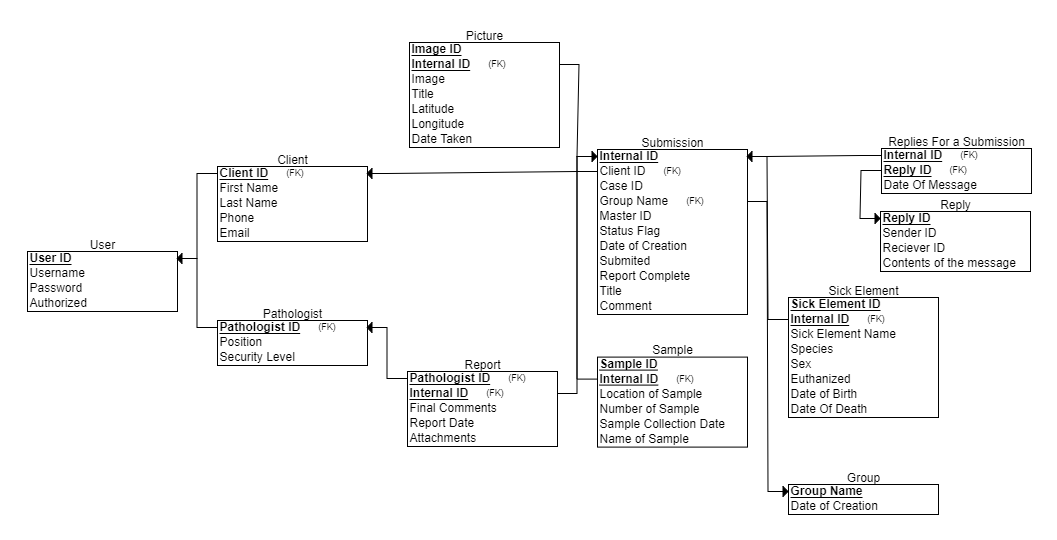
\includegraphics[height=8cm]{Beta_ERD.png}
\end{center}
\captionof{figure}{Beta ER Diagram}

\begin{center}
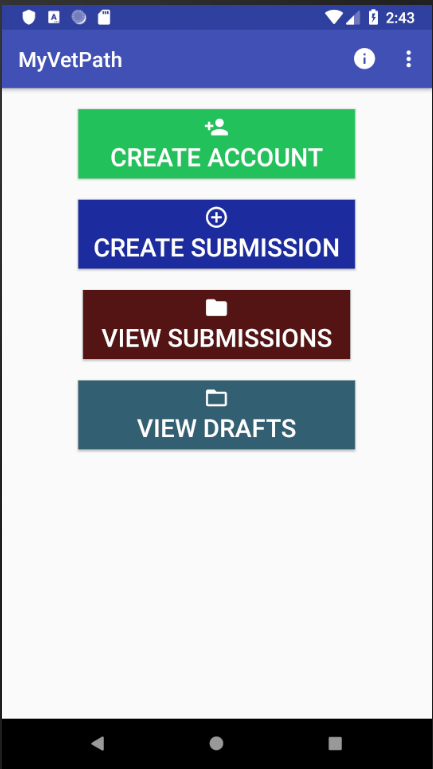
\includegraphics[height=8cm]{home.png}
\end{center}
\captionof{figure}{Home Screen}

\begin{center}
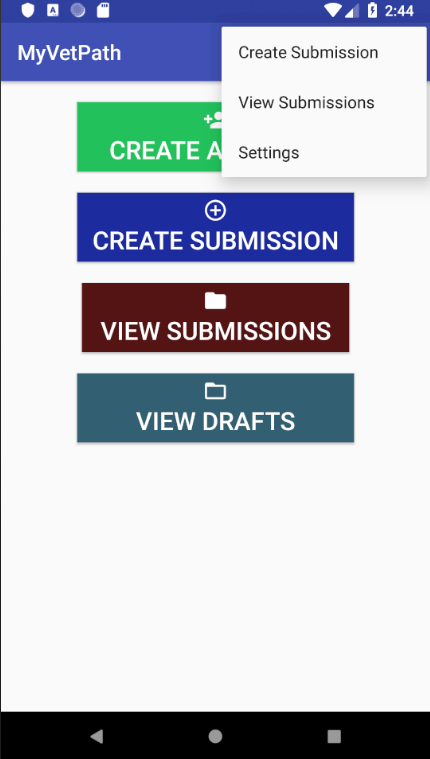
\includegraphics[height=8cm]{toolbar.png}
\end{center}
\captionof{figure}{Toolbar}

\begin{center}
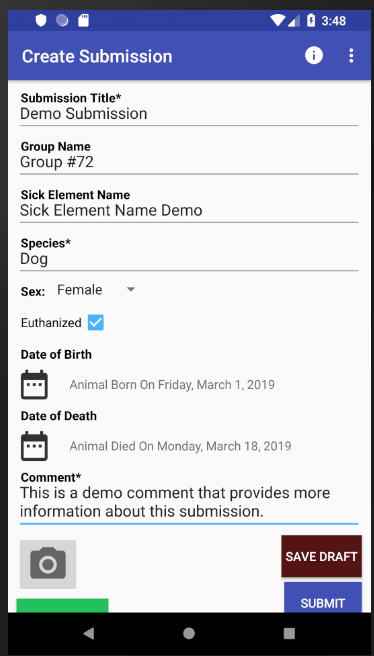
\includegraphics[height=8cm]{Beta_create_sub_1.png}
\end{center}
\captionof{figure}{Create Submissions Screen}

\begin{center}
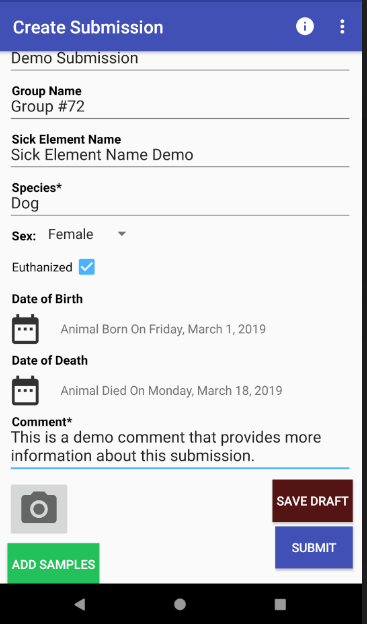
\includegraphics[height=8cm]{Beta_create_sub_2.png}
\end{center}
\captionof{figure}{Create Submissions Screen (Part 2)}

\begin{center}
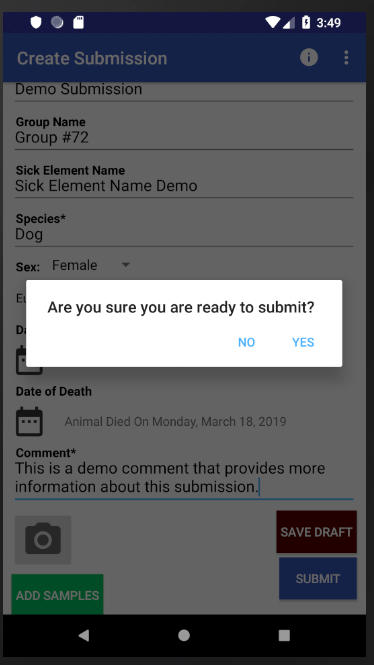
\includegraphics[height=8cm]{Beta_create_sub_3.png}
\end{center}
\captionof{figure}{Create Submissions Screen (Part 3)}


\begin{center}
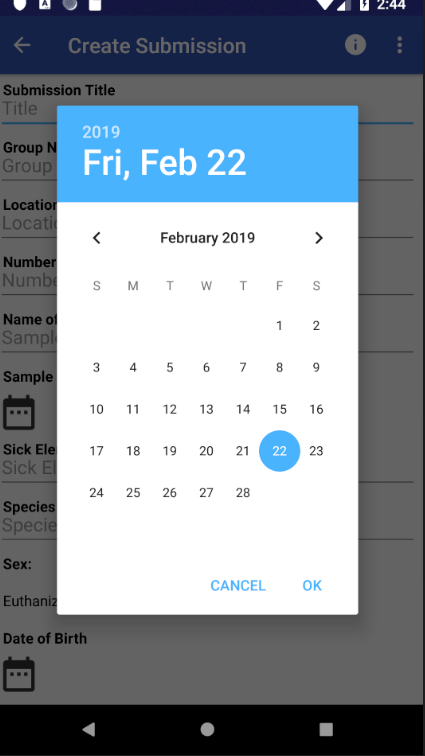
\includegraphics[height=8cm]{datePickerFragment.png}
\end{center}
\captionof{figure}{Date Picker}

\begin{center}
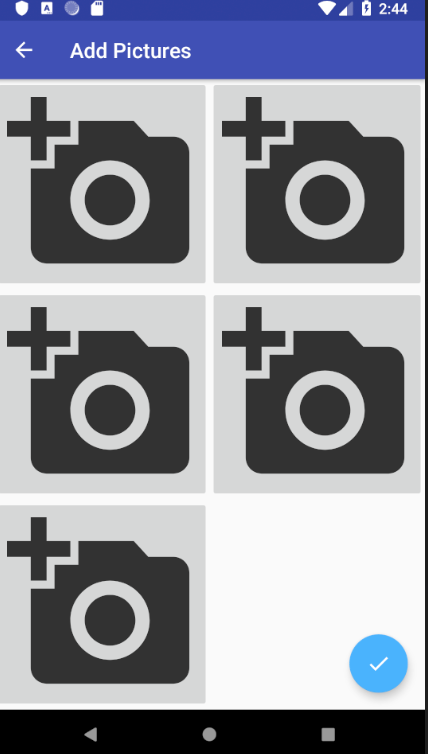
\includegraphics[height=8cm]{add_pictures.png}
\end{center}
\captionof{figure}{Add Pictures Screen}

\begin{center}
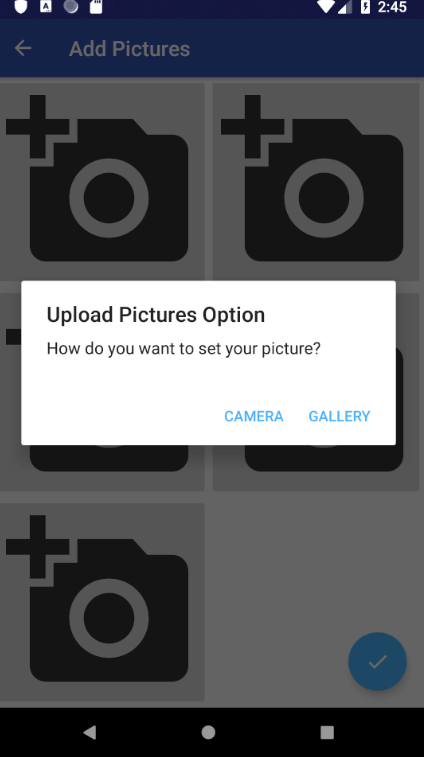
\includegraphics[height=8cm]{add_pictures_choice.png}
\end{center}
\captionof{figure}{Add Pictures Prompt}

\begin{center}
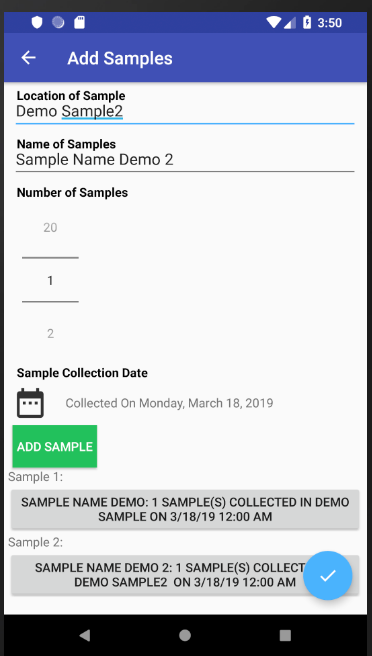
\includegraphics[height=8cm]{Beta_Add_samples.png}
\end{center}
\captionof{figure}{Add Samples Screen}

\begin{center}
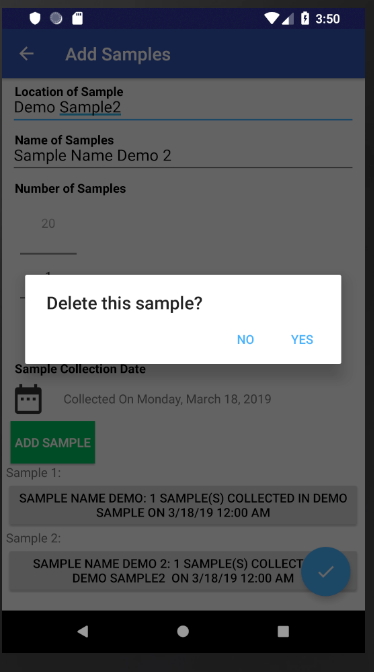
\includegraphics[height=8cm]{Beta_Add_samples_2.png}
\end{center}
\captionof{figure}{Add Samples Screen (Part 2)}

\begin{center}
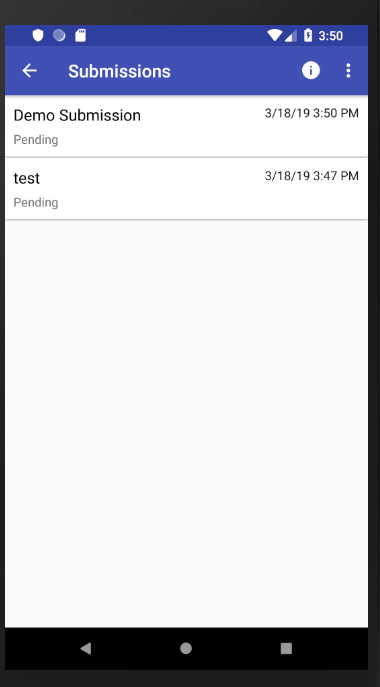
\includegraphics[height=8cm]{Beta_submissions.png}
\end{center}
\captionof{figure}{View Submissions Screen}

\begin{center}
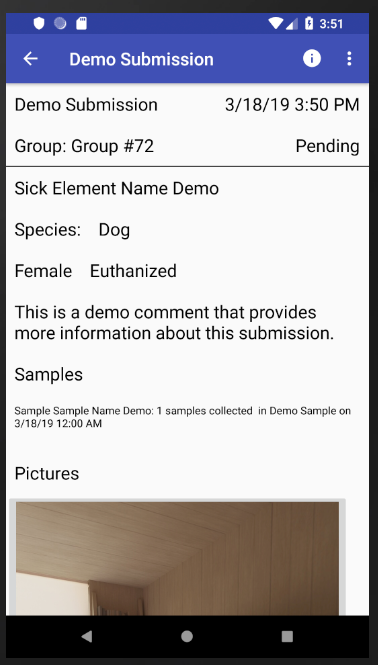
\includegraphics[height=8cm]{Beta_detailed_submission_1.png}
\end{center}
\captionof{figure}{Detailed Submissions Screen}

\begin{center}
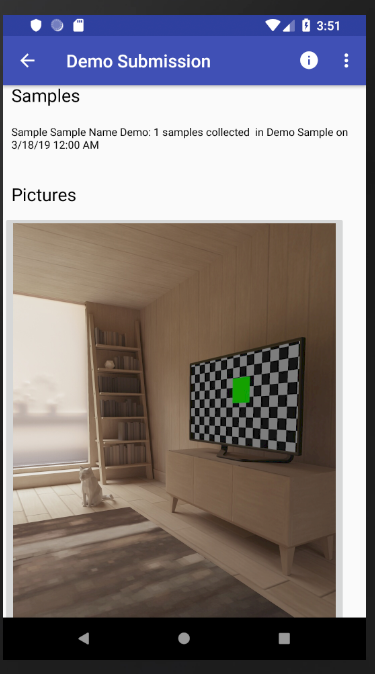
\includegraphics[height=8cm]{Beta_detailed_submission_2.png}
\end{center}
\captionof{figure}{Detailed Submissions Screen (Part 2)}

\begin{center}
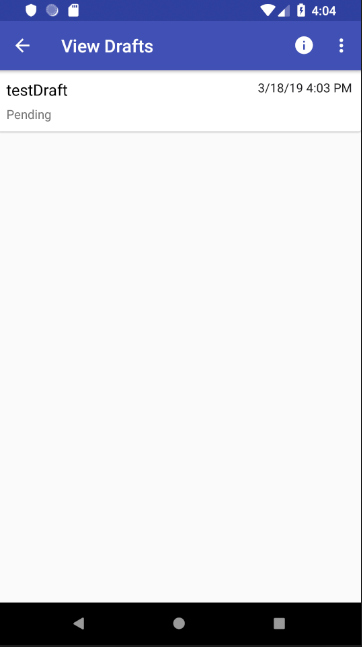
\includegraphics[height=8cm]{Beta_test_draft.png}
\end{center}
\captionof{figure}{View Drafts Screen}

\begin{center}
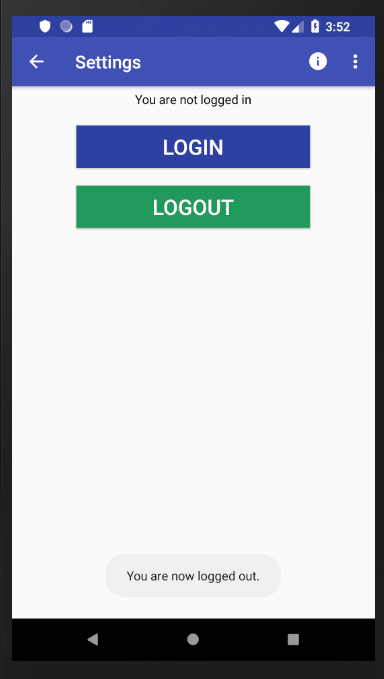
\includegraphics[height=8cm]{Beta_settings_1.png}
\end{center}
\captionof{figure}{Settings Screen (Logged out)}

\begin{center}
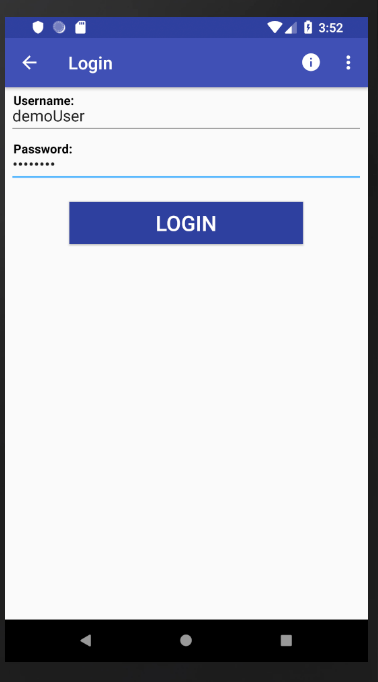
\includegraphics[height=8cm]{Beta_settings_2.png}
\end{center}
\captionof{figure}{Log In Screen}

\begin{center}
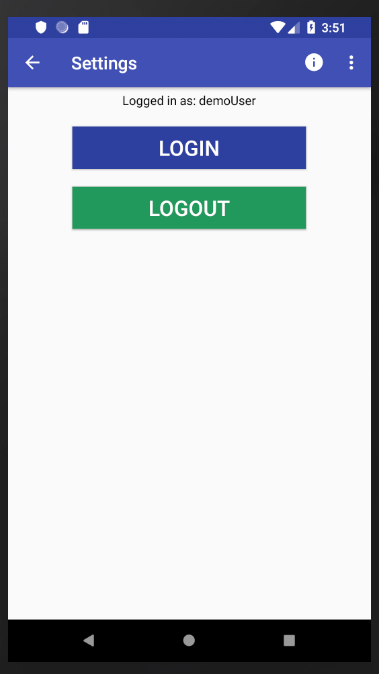
\includegraphics[height=8cm]{Beta_settings_3.png}
\end{center}
\captionof{figure}{Settings Screen (Logged In)}

\begin{center}
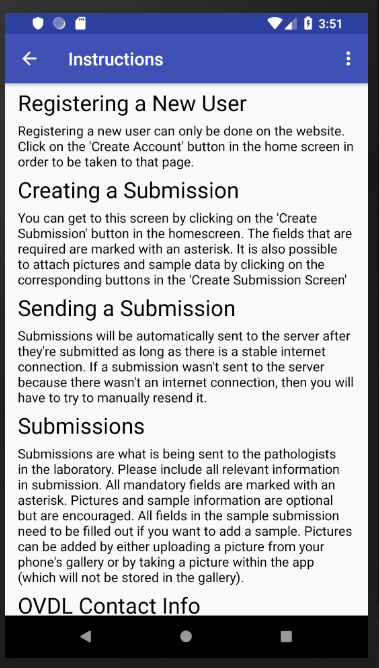
\includegraphics[height=8cm]{Beta_inscructions_1.png}
\end{center}
\captionof{figure}{Instructions Screen}

\begin{center}
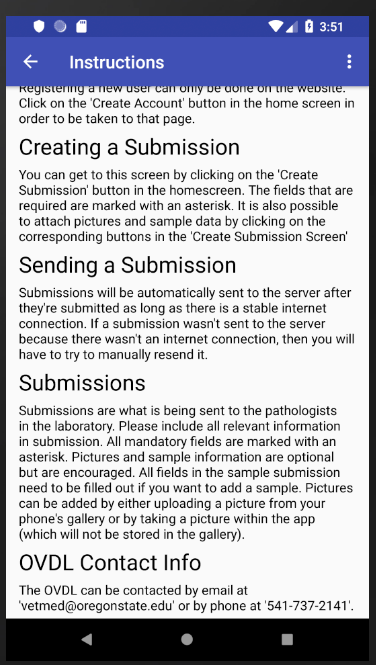
\includegraphics[height=8cm]{Beta_instructions_2.png}
\end{center}
\captionof{figure}{Instructions Screen (Part 2)}

\begin{center}
    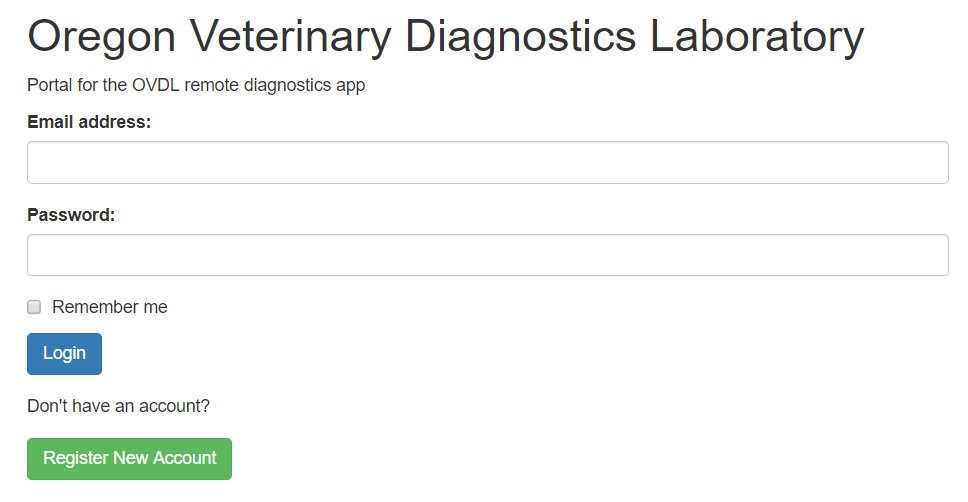
\includegraphics[height=6cm]{login_web.png}
\end{center}
\captionof{figure}{Website Login Screen}

\begin{center}
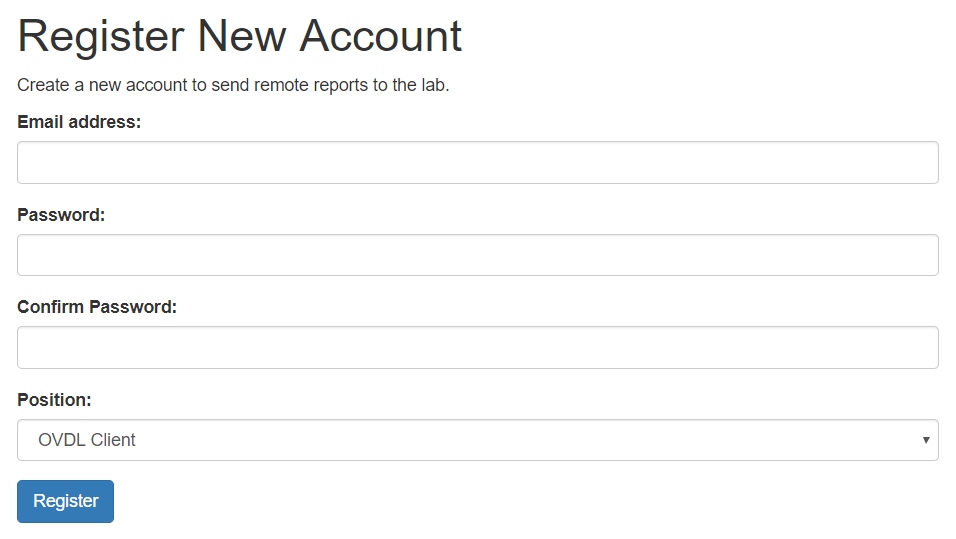
\includegraphics[height=6cm]{register_web.png}
\end{center}
\captionof{figure}{Website Registration Screen}



\end{document}